% Created by tikzDevice version 0.12.3 on 2019-12-13 14:56:45
% !TEX encoding = UTF-8 Unicode
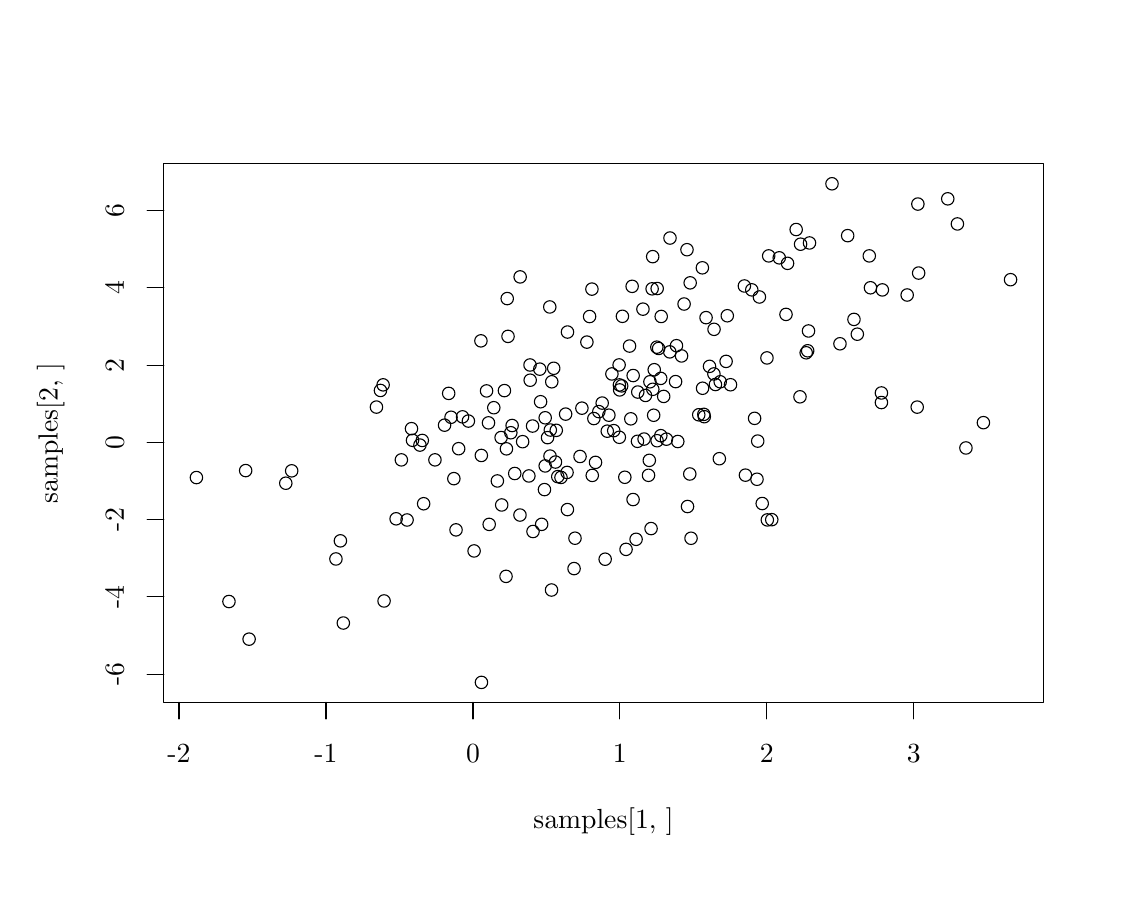
\begin{tikzpicture}[x=1pt,y=1pt]
\definecolor{fillColor}{RGB}{255,255,255}
\path[use as bounding box,fill=fillColor,fill opacity=0.00] (0,0) rectangle (392.13,304.99);
\begin{scope}
\path[clip] ( 49.20, 61.20) rectangle (366.93,255.79);
\definecolor{drawColor}{RGB}{0,0,0}

\path[draw=drawColor,line width= 0.4pt,line join=round,line cap=round] (242.49,165.11) circle (  2.25);

\path[draw=drawColor,line width= 0.4pt,line join=round,line cap=round] (281.85,188.23) circle (  2.25);

\path[draw=drawColor,line width= 0.4pt,line join=round,line cap=round] (133.13,127.52) circle (  2.25);

\path[draw=drawColor,line width= 0.4pt,line join=round,line cap=round] (267.76,222.52) circle (  2.25);

\path[draw=drawColor,line width= 0.4pt,line join=round,line cap=round] (182.60,122.93) circle (  2.25);

\path[draw=drawColor,line width= 0.4pt,line join=round,line cap=round] (163.97, 68.41) circle (  2.25);

\path[draw=drawColor,line width= 0.4pt,line join=round,line cap=round] ( 60.97,142.42) circle (  2.25);

\path[draw=drawColor,line width= 0.4pt,line join=round,line cap=round] (182.44,161.04) circle (  2.25);

\path[draw=drawColor,line width= 0.4pt,line join=round,line cap=round] (152.98,164.21) circle (  2.25);

\path[draw=drawColor,line width= 0.4pt,line join=round,line cap=round] (216.22,116.48) circle (  2.25);

\path[draw=drawColor,line width= 0.4pt,line join=round,line cap=round] (244.33,165.26) circle (  2.25);

\path[draw=drawColor,line width= 0.4pt,line join=round,line cap=round] (111.39,113.01) circle (  2.25);

\path[draw=drawColor,line width= 0.4pt,line join=round,line cap=round] (206.38,166.25) circle (  2.25);

\path[draw=drawColor,line width= 0.4pt,line join=round,line cap=round] (141.74,154.16) circle (  2.25);

\path[draw=drawColor,line width= 0.4pt,line join=round,line cap=round] (321.67,241.25) circle (  2.25);

\path[draw=drawColor,line width= 0.4pt,line join=round,line cap=round] (227.47,210.73) circle (  2.25);

\path[draw=drawColor,line width= 0.4pt,line join=round,line cap=round] (222.33,203.28) circle (  2.25);

\path[draw=drawColor,line width= 0.4pt,line join=round,line cap=round] (174.58,158.62) circle (  2.25);

\path[draw=drawColor,line width= 0.4pt,line join=round,line cap=round] (261.65,210.25) circle (  2.25);

\path[draw=drawColor,line width= 0.4pt,line join=round,line cap=round] (214.64,175.55) circle (  2.25);

\path[draw=drawColor,line width= 0.4pt,line join=round,line cap=round] (172.27,173.84) circle (  2.25);

\path[draw=drawColor,line width= 0.4pt,line join=round,line cap=round] (267.14,185.65) circle (  2.25);

\path[draw=drawColor,line width= 0.4pt,line join=round,line cap=round] (339.04,153.12) circle (  2.25);

\path[draw=drawColor,line width= 0.4pt,line join=round,line cap=round] (204.01,143.20) circle (  2.25);

\path[draw=drawColor,line width= 0.4pt,line join=round,line cap=round] (168.43,167.66) circle (  2.25);

\path[draw=drawColor,line width= 0.4pt,line join=round,line cap=round] (187.00,146.62) circle (  2.25);

\path[draw=drawColor,line width= 0.4pt,line join=round,line cap=round] (250.25,177.03) circle (  2.25);

\path[draw=drawColor,line width= 0.4pt,line join=round,line cap=round] (225.89,174.32) circle (  2.25);

\path[draw=drawColor,line width= 0.4pt,line join=round,line cap=round] (243.87,174.70) circle (  2.25);

\path[draw=drawColor,line width= 0.4pt,line join=round,line cap=round] (258.98,211.65) circle (  2.25);

\path[draw=drawColor,line width= 0.4pt,line join=round,line cap=round] (234.91,155.45) circle (  2.25);

\path[draw=drawColor,line width= 0.4pt,line join=round,line cap=round] (191.00,159.49) circle (  2.25);

\path[draw=drawColor,line width= 0.4pt,line join=round,line cap=round] (264.41,207.67) circle (  2.25);

\path[draw=drawColor,line width= 0.4pt,line join=round,line cap=round] (296.30,229.84) circle (  2.25);

\path[draw=drawColor,line width= 0.4pt,line join=round,line cap=round] (187.85,156.85) circle (  2.25);

\path[draw=drawColor,line width= 0.4pt,line join=round,line cap=round] (234.44,190.07) circle (  2.25);

\path[draw=drawColor,line width= 0.4pt,line join=round,line cap=round] (177.95,214.93) circle (  2.25);

\path[draw=drawColor,line width= 0.4pt,line join=round,line cap=round] (308.50,169.53) circle (  2.25);

\path[draw=drawColor,line width= 0.4pt,line join=round,line cap=round] (228.92,200.63) circle (  2.25);

\path[draw=drawColor,line width= 0.4pt,line join=round,line cap=round] (232.02,187.84) circle (  2.25);

\path[draw=drawColor,line width= 0.4pt,line join=round,line cap=round] (226.20,164.94) circle (  2.25);

\path[draw=drawColor,line width= 0.4pt,line join=round,line cap=round] (217.48,189.94) circle (  2.25);

\path[draw=drawColor,line width= 0.4pt,line join=round,line cap=round] (139.06,155.89) circle (  2.25);

\path[draw=drawColor,line width= 0.4pt,line join=round,line cap=round] (213.82,175.90) circle (  2.25);

\path[draw=drawColor,line width= 0.4pt,line join=round,line cap=round] (173.57,193.44) circle (  2.25);

\path[draw=drawColor,line width= 0.4pt,line join=round,line cap=round] (228.78,157.56) circle (  2.25);

\path[draw=drawColor,line width= 0.4pt,line join=round,line cap=round] (188.66,204.07) circle (  2.25);

\path[draw=drawColor,line width= 0.4pt,line join=round,line cap=round] (152.13,172.84) circle (  2.25);

\path[draw=drawColor,line width= 0.4pt,line join=round,line cap=round] (321.95,216.32) circle (  2.25);

\path[draw=drawColor,line width= 0.4pt,line join=round,line cap=round] (317.80,208.39) circle (  2.25);

\path[draw=drawColor,line width= 0.4pt,line join=round,line cap=round] (219.85,120.11) circle (  2.25);

\path[draw=drawColor,line width= 0.4pt,line join=round,line cap=round] (218.79,179.29) circle (  2.25);

\path[draw=drawColor,line width= 0.4pt,line join=round,line cap=round] (223.24,172.10) circle (  2.25);

\path[draw=drawColor,line width= 0.4pt,line join=round,line cap=round] (127.48,173.90) circle (  2.25);

\path[draw=drawColor,line width= 0.4pt,line join=round,line cap=round] (248.52,176.05) circle (  2.25);

\path[draw=drawColor,line width= 0.4pt,line join=round,line cap=round] (218.76,134.48) circle (  2.25);

\path[draw=drawColor,line width= 0.4pt,line join=round,line cap=round] (263.54,141.81) circle (  2.25);

\path[draw=drawColor,line width= 0.4pt,line join=round,line cap=round] (274.02,201.38) circle (  2.25);

\path[draw=drawColor,line width= 0.4pt,line join=round,line cap=round] ( 80.01, 84.03) circle (  2.25);

\path[draw=drawColor,line width= 0.4pt,line join=round,line cap=round] (175.05,161.23) circle (  2.25);

\path[draw=drawColor,line width= 0.4pt,line join=round,line cap=round] (225.26,123.99) circle (  2.25);

\path[draw=drawColor,line width= 0.4pt,line join=round,line cap=round] (308.84,210.23) circle (  2.25);

\path[draw=drawColor,line width= 0.4pt,line join=round,line cap=round] (171.07,156.88) circle (  2.25);

\path[draw=drawColor,line width= 0.4pt,line join=round,line cap=round] (194.90,144.27) circle (  2.25);

\path[draw=drawColor,line width= 0.4pt,line join=round,line cap=round] ( 72.74, 97.63) circle (  2.25);

\path[draw=drawColor,line width= 0.4pt,line join=round,line cap=round] (222.74,156.34) circle (  2.25);

\path[draw=drawColor,line width= 0.4pt,line join=round,line cap=round] (211.11,179.86) circle (  2.25);

\path[draw=drawColor,line width= 0.4pt,line join=round,line cap=round] (225.85,222.25) circle (  2.25);

\path[draw=drawColor,line width= 0.4pt,line join=round,line cap=round] (166.52,162.19) circle (  2.25);

\path[draw=drawColor,line width= 0.4pt,line join=round,line cap=round] (321.43,167.88) circle (  2.25);

\path[draw=drawColor,line width= 0.4pt,line join=round,line cap=round] (248.01,195.99) circle (  2.25);

\path[draw=drawColor,line width= 0.4pt,line join=round,line cap=round] (229.82,171.74) circle (  2.25);

\path[draw=drawColor,line width= 0.4pt,line join=round,line cap=round] (210.02,164.96) circle (  2.25);

\path[draw=drawColor,line width= 0.4pt,line join=round,line cap=round] (213.80,156.98) circle (  2.25);

\path[draw=drawColor,line width= 0.4pt,line join=round,line cap=round] (157.13,164.36) circle (  2.25);

\path[draw=drawColor,line width= 0.4pt,line join=round,line cap=round] (189.29,101.79) circle (  2.25);

\path[draw=drawColor,line width= 0.4pt,line join=round,line cap=round] (208.67,112.92) circle (  2.25);

\path[draw=drawColor,line width= 0.4pt,line join=round,line cap=round] (142.59,155.83) circle (  2.25);

\path[draw=drawColor,line width= 0.4pt,line join=round,line cap=round] (203.89,210.52) circle (  2.25);

\path[draw=drawColor,line width= 0.4pt,line join=round,line cap=round] (259.36,143.30) circle (  2.25);

\path[draw=drawColor,line width= 0.4pt,line join=round,line cap=round] (128.44,175.92) circle (  2.25);

\path[draw=drawColor,line width= 0.4pt,line join=round,line cap=round] (155.74,152.85) circle (  2.25);

\path[draw=drawColor,line width= 0.4pt,line join=round,line cap=round] (211.77,159.37) circle (  2.25);

\path[draw=drawColor,line width= 0.4pt,line join=round,line cap=round] (290.64,248.58) circle (  2.25);

\path[draw=drawColor,line width= 0.4pt,line join=round,line cap=round] (178.85,155.39) circle (  2.25);

\path[draw=drawColor,line width= 0.4pt,line join=round,line cap=round] (238.24,224.76) circle (  2.25);

\path[draw=drawColor,line width= 0.4pt,line join=round,line cap=round] (165.81,173.73) circle (  2.25);

\path[draw=drawColor,line width= 0.4pt,line join=round,line cap=round] (213.91,174.09) circle (  2.25);

\path[draw=drawColor,line width= 0.4pt,line join=round,line cap=round] (191.55,142.76) circle (  2.25);

\path[draw=drawColor,line width= 0.4pt,line join=round,line cap=round] (345.35,162.26) circle (  2.25);

\path[draw=drawColor,line width= 0.4pt,line join=round,line cap=round] (154.78,123.52) circle (  2.25);

\path[draw=drawColor,line width= 0.4pt,line join=round,line cap=round] (113.00,119.55) circle (  2.25);

\path[draw=drawColor,line width= 0.4pt,line join=round,line cap=round] (161.31,115.91) circle (  2.25);

\path[draw=drawColor,line width= 0.4pt,line join=round,line cap=round] (282.15,195.39) circle (  2.25);

\path[draw=drawColor,line width= 0.4pt,line join=round,line cap=round] ( 93.27,140.38) circle (  2.25);

\path[draw=drawColor,line width= 0.4pt,line join=round,line cap=round] (293.52,190.76) circle (  2.25);

\path[draw=drawColor,line width= 0.4pt,line join=round,line cap=round] (185.73,125.52) circle (  2.25);

\path[draw=drawColor,line width= 0.4pt,line join=round,line cap=round] (209.43,159.18) circle (  2.25);

\path[draw=drawColor,line width= 0.4pt,line join=round,line cap=round] (176.00,143.89) circle (  2.25);

\path[draw=drawColor,line width= 0.4pt,line join=round,line cap=round] (252.37,184.40) circle (  2.25);

\path[draw=drawColor,line width= 0.4pt,line join=round,line cap=round] (173.28,207.10) circle (  2.25);

\path[draw=drawColor,line width= 0.4pt,line join=round,line cap=round] (355.16,213.92) circle (  2.25);

\path[draw=drawColor,line width= 0.4pt,line join=round,line cap=round] ( 78.77,144.94) circle (  2.25);

\path[draw=drawColor,line width= 0.4pt,line join=round,line cap=round] (186.74,138.07) circle (  2.25);

\path[draw=drawColor,line width= 0.4pt,line join=round,line cap=round] (128.78, 97.83) circle (  2.25);

\path[draw=drawColor,line width= 0.4pt,line join=round,line cap=round] (199.59,150.04) circle (  2.25);

\path[draw=drawColor,line width= 0.4pt,line join=round,line cap=round] (205.19,147.91) circle (  2.25);

\path[draw=drawColor,line width= 0.4pt,line join=round,line cap=round] (304.54,211.00) circle (  2.25);

\path[draw=drawColor,line width= 0.4pt,line join=round,line cap=round] (332.47,243.14) circle (  2.25);

\path[draw=drawColor,line width= 0.4pt,line join=round,line cap=round] (126.03,167.89) circle (  2.25);

\path[draw=drawColor,line width= 0.4pt,line join=round,line cap=round] (239.70,120.49) circle (  2.25);

\path[draw=drawColor,line width= 0.4pt,line join=round,line cap=round] (246.38,182.61) circle (  2.25);

\path[draw=drawColor,line width= 0.4pt,line join=round,line cap=round] (171.29,132.52) circle (  2.25);

\path[draw=drawColor,line width= 0.4pt,line join=round,line cap=round] (188.74,150.18) circle (  2.25);

\path[draw=drawColor,line width= 0.4pt,line join=round,line cap=round] (207.60,169.34) circle (  2.25);

\path[draw=drawColor,line width= 0.4pt,line join=round,line cap=round] (282.51,227.20) circle (  2.25);

\path[draw=drawColor,line width= 0.4pt,line join=round,line cap=round] (187.00,164.02) circle (  2.25);

\path[draw=drawColor,line width= 0.4pt,line join=round,line cap=round] (220.35,155.52) circle (  2.25);

\path[draw=drawColor,line width= 0.4pt,line join=round,line cap=round] (299.79,194.23) circle (  2.25);

\path[draw=drawColor,line width= 0.4pt,line join=round,line cap=round] (239.25,143.71) circle (  2.25);

\path[draw=drawColor,line width= 0.4pt,line join=round,line cap=round] (169.72,141.20) circle (  2.25);

\path[draw=drawColor,line width= 0.4pt,line join=round,line cap=round] (262.67,163.82) circle (  2.25);

\path[draw=drawColor,line width= 0.4pt,line join=round,line cap=round] (197.77,120.51) circle (  2.25);

\path[draw=drawColor,line width= 0.4pt,line join=round,line cap=round] (220.46,173.33) circle (  2.25);

\path[draw=drawColor,line width= 0.4pt,line join=round,line cap=round] (234.12,177.09) circle (  2.25);

\path[draw=drawColor,line width= 0.4pt,line join=round,line cap=round] (279.07,171.60) circle (  2.25);

\path[draw=drawColor,line width= 0.4pt,line join=round,line cap=round] (181.52,183.10) circle (  2.25);

\path[draw=drawColor,line width= 0.4pt,line join=round,line cap=round] (335.96,234.07) circle (  2.25);

\path[draw=drawColor,line width= 0.4pt,line join=round,line cap=round] (263.80,155.60) circle (  2.25);

\path[draw=drawColor,line width= 0.4pt,line join=round,line cap=round] (190.72,148.03) circle (  2.25);

\path[draw=drawColor,line width= 0.4pt,line join=round,line cap=round] (213.71,183.12) circle (  2.25);

\path[draw=drawColor,line width= 0.4pt,line join=round,line cap=round] (227.44,155.73) circle (  2.25);

\path[draw=drawColor,line width= 0.4pt,line join=round,line cap=round] (249.93,149.23) circle (  2.25);

\path[draw=drawColor,line width= 0.4pt,line join=round,line cap=round] (197.43,109.53) circle (  2.25);

\path[draw=drawColor,line width= 0.4pt,line join=round,line cap=round] (238.43,131.96) circle (  2.25);

\path[draw=drawColor,line width= 0.4pt,line join=round,line cap=round] (195.06,195.01) circle (  2.25);

\path[draw=drawColor,line width= 0.4pt,line join=round,line cap=round] (173.00,152.80) circle (  2.25);

\path[draw=drawColor,line width= 0.4pt,line join=round,line cap=round] (150.64,161.36) circle (  2.25);

\path[draw=drawColor,line width= 0.4pt,line join=round,line cap=round] (185.34,169.82) circle (  2.25);

\path[draw=drawColor,line width= 0.4pt,line join=round,line cap=round] (271.58,221.82) circle (  2.25);

\path[draw=drawColor,line width= 0.4pt,line join=round,line cap=round] (308.50,172.99) circle (  2.25);

\path[draw=drawColor,line width= 0.4pt,line join=round,line cap=round] (163.78,191.82) circle (  2.25);

\path[draw=drawColor,line width= 0.4pt,line join=round,line cap=round] (181.58,177.60) circle (  2.25);

\path[draw=drawColor,line width= 0.4pt,line join=round,line cap=round] (204.59,163.75) circle (  2.25);

\path[draw=drawColor,line width= 0.4pt,line join=round,line cap=round] (252.80,200.89) circle (  2.25);

\path[draw=drawColor,line width= 0.4pt,line join=round,line cap=round] (268.87,127.20) circle (  2.25);

\path[draw=drawColor,line width= 0.4pt,line join=round,line cap=round] (194.39,165.35) circle (  2.25);

\path[draw=drawColor,line width= 0.4pt,line join=round,line cap=round] (215.78,142.53) circle (  2.25);

\path[draw=drawColor,line width= 0.4pt,line join=round,line cap=round] (135.03,148.81) circle (  2.25);

\path[draw=drawColor,line width= 0.4pt,line join=round,line cap=round] (247.97,179.86) circle (  2.25);

\path[draw=drawColor,line width= 0.4pt,line join=round,line cap=round] (226.40,181.39) circle (  2.25);

\path[draw=drawColor,line width= 0.4pt,line join=round,line cap=round] (218.42,211.52) circle (  2.25);

\path[draw=drawColor,line width= 0.4pt,line join=round,line cap=round] (138.69,160.09) circle (  2.25);

\path[draw=drawColor,line width= 0.4pt,line join=round,line cap=round] (188.85,159.60) circle (  2.25);

\path[draw=drawColor,line width= 0.4pt,line join=round,line cap=round] (265.42,133.04) circle (  2.25);

\path[draw=drawColor,line width= 0.4pt,line join=round,line cap=round] (163.93,150.41) circle (  2.25);

\path[draw=drawColor,line width= 0.4pt,line join=round,line cap=round] (172.85,106.72) circle (  2.25);

\path[draw=drawColor,line width= 0.4pt,line join=round,line cap=round] (189.38,177.03) circle (  2.25);

\path[draw=drawColor,line width= 0.4pt,line join=round,line cap=round] (224.85,177.03) circle (  2.25);

\path[draw=drawColor,line width= 0.4pt,line join=round,line cap=round] (224.34,143.24) circle (  2.25);

\path[draw=drawColor,line width= 0.4pt,line join=round,line cap=round] (159.25,162.84) circle (  2.25);

\path[draw=drawColor,line width= 0.4pt,line join=round,line cap=round] (185.05,181.60) circle (  2.25);

\path[draw=drawColor,line width= 0.4pt,line join=round,line cap=round] (154.00,142.03) circle (  2.25);

\path[draw=drawColor,line width= 0.4pt,line join=round,line cap=round] (281.31,187.51) circle (  2.25);

\path[draw=drawColor,line width= 0.4pt,line join=round,line cap=round] (143.08,132.96) circle (  2.25);

\path[draw=drawColor,line width= 0.4pt,line join=round,line cap=round] (202.07,191.37) circle (  2.25);

\path[draw=drawColor,line width= 0.4pt,line join=round,line cap=round] (217.94,163.64) circle (  2.25);

\path[draw=drawColor,line width= 0.4pt,line join=round,line cap=round] (236.28,186.37) circle (  2.25);

\path[draw=drawColor,line width= 0.4pt,line join=round,line cap=round] (279.28,226.75) circle (  2.25);

\path[draw=drawColor,line width= 0.4pt,line join=round,line cap=round] ( 95.40,144.85) circle (  2.25);

\path[draw=drawColor,line width= 0.4pt,line join=round,line cap=round] (203.05,200.61) circle (  2.25);

\path[draw=drawColor,line width= 0.4pt,line join=round,line cap=round] (195.03,130.85) circle (  2.25);

\path[draw=drawColor,line width= 0.4pt,line join=round,line cap=round] (214.91,200.69) circle (  2.25);

\path[draw=drawColor,line width= 0.4pt,line join=round,line cap=round] (147.17,148.82) circle (  2.25);

\path[draw=drawColor,line width= 0.4pt,line join=round,line cap=round] (244.49,164.42) circle (  2.25);

\path[draw=drawColor,line width= 0.4pt,line join=round,line cap=round] (166.76,125.50) circle (  2.25);

\path[draw=drawColor,line width= 0.4pt,line join=round,line cap=round] (239.39,212.78) circle (  2.25);

\path[draw=drawColor,line width= 0.4pt,line join=round,line cap=round] (304.11,222.52) circle (  2.25);

\path[draw=drawColor,line width= 0.4pt,line join=round,line cap=round] (228.75,178.26) circle (  2.25);

\path[draw=drawColor,line width= 0.4pt,line join=round,line cap=round] (227.99,189.07) circle (  2.25);

\path[draw=drawColor,line width= 0.4pt,line join=round,line cap=round] (267.27,127.12) circle (  2.25);

\path[draw=drawColor,line width= 0.4pt,line join=round,line cap=round] (277.69,232.05) circle (  2.25);

\path[draw=drawColor,line width= 0.4pt,line join=round,line cap=round] (227.35,189.54) circle (  2.25);

\path[draw=drawColor,line width= 0.4pt,line join=round,line cap=round] (298.58,199.57) circle (  2.25);

\path[draw=drawColor,line width= 0.4pt,line join=round,line cap=round] (232.10,228.98) circle (  2.25);

\path[draw=drawColor,line width= 0.4pt,line join=round,line cap=round] (274.58,219.83) circle (  2.25);

\path[draw=drawColor,line width= 0.4pt,line join=round,line cap=round] (137.09,127.09) circle (  2.25);

\path[draw=drawColor,line width= 0.4pt,line join=round,line cap=round] (243.80,218.21) circle (  2.25);

\path[draw=drawColor,line width= 0.4pt,line join=round,line cap=round] (224.62,148.64) circle (  2.25);

\path[draw=drawColor,line width= 0.4pt,line join=round,line cap=round] (225.64,210.62) circle (  2.25);

\path[draw=drawColor,line width= 0.4pt,line join=round,line cap=round] (253.96,175.96) circle (  2.25);

\path[draw=drawColor,line width= 0.4pt,line join=round,line cap=round] (181.11,143.00) circle (  2.25);

\path[draw=drawColor,line width= 0.4pt,line join=round,line cap=round] (200.27,167.50) circle (  2.25);

\path[draw=drawColor,line width= 0.4pt,line join=round,line cap=round] (177.89,128.88) circle (  2.25);

\path[draw=drawColor,line width= 0.4pt,line join=round,line cap=round] (230.81,156.30) circle (  2.25);

\path[draw=drawColor,line width= 0.4pt,line join=round,line cap=round] (192.71,142.47) circle (  2.25);

\path[draw=drawColor,line width= 0.4pt,line join=round,line cap=round] (245.13,200.21) circle (  2.25);

\path[draw=drawColor,line width= 0.4pt,line join=round,line cap=round] (114.06, 89.86) circle (  2.25);

\path[draw=drawColor,line width= 0.4pt,line join=round,line cap=round] (237.19,205.13) circle (  2.25);

\path[draw=drawColor,line width= 0.4pt,line join=round,line cap=round] (190.08,181.91) circle (  2.25);
\end{scope}
\begin{scope}
\path[clip] (  0.00,  0.00) rectangle (392.13,304.99);
\definecolor{drawColor}{RGB}{0,0,0}

\path[draw=drawColor,line width= 0.4pt,line join=round,line cap=round] ( 54.69, 61.20) -- (320.21, 61.20);

\path[draw=drawColor,line width= 0.4pt,line join=round,line cap=round] ( 54.69, 61.20) -- ( 54.69, 55.20);

\path[draw=drawColor,line width= 0.4pt,line join=round,line cap=round] (107.79, 61.20) -- (107.79, 55.20);

\path[draw=drawColor,line width= 0.4pt,line join=round,line cap=round] (160.90, 61.20) -- (160.90, 55.20);

\path[draw=drawColor,line width= 0.4pt,line join=round,line cap=round] (214.00, 61.20) -- (214.00, 55.20);

\path[draw=drawColor,line width= 0.4pt,line join=round,line cap=round] (267.11, 61.20) -- (267.11, 55.20);

\path[draw=drawColor,line width= 0.4pt,line join=round,line cap=round] (320.21, 61.20) -- (320.21, 55.20);

\node[text=drawColor,anchor=base,inner sep=0pt, outer sep=0pt, scale=  1.00] at ( 54.69, 39.60) {-2};

\node[text=drawColor,anchor=base,inner sep=0pt, outer sep=0pt, scale=  1.00] at (107.79, 39.60) {-1};

\node[text=drawColor,anchor=base,inner sep=0pt, outer sep=0pt, scale=  1.00] at (160.90, 39.60) {0};

\node[text=drawColor,anchor=base,inner sep=0pt, outer sep=0pt, scale=  1.00] at (214.00, 39.60) {1};

\node[text=drawColor,anchor=base,inner sep=0pt, outer sep=0pt, scale=  1.00] at (267.11, 39.60) {2};

\node[text=drawColor,anchor=base,inner sep=0pt, outer sep=0pt, scale=  1.00] at (320.21, 39.60) {3};

\path[draw=drawColor,line width= 0.4pt,line join=round,line cap=round] ( 49.20, 71.37) -- ( 49.20,238.90);

\path[draw=drawColor,line width= 0.4pt,line join=round,line cap=round] ( 49.20, 71.37) -- ( 43.20, 71.37);

\path[draw=drawColor,line width= 0.4pt,line join=round,line cap=round] ( 49.20, 99.29) -- ( 43.20, 99.29);

\path[draw=drawColor,line width= 0.4pt,line join=round,line cap=round] ( 49.20,127.22) -- ( 43.20,127.22);

\path[draw=drawColor,line width= 0.4pt,line join=round,line cap=round] ( 49.20,155.14) -- ( 43.20,155.14);

\path[draw=drawColor,line width= 0.4pt,line join=round,line cap=round] ( 49.20,183.06) -- ( 43.20,183.06);

\path[draw=drawColor,line width= 0.4pt,line join=round,line cap=round] ( 49.20,210.98) -- ( 43.20,210.98);

\path[draw=drawColor,line width= 0.4pt,line join=round,line cap=round] ( 49.20,238.90) -- ( 43.20,238.90);

\node[text=drawColor,rotate= 90.00,anchor=base,inner sep=0pt, outer sep=0pt, scale=  1.00] at ( 34.80, 71.37) {-6};

\node[text=drawColor,rotate= 90.00,anchor=base,inner sep=0pt, outer sep=0pt, scale=  1.00] at ( 34.80, 99.29) {-4};

\node[text=drawColor,rotate= 90.00,anchor=base,inner sep=0pt, outer sep=0pt, scale=  1.00] at ( 34.80,127.22) {-2};

\node[text=drawColor,rotate= 90.00,anchor=base,inner sep=0pt, outer sep=0pt, scale=  1.00] at ( 34.80,155.14) {0};

\node[text=drawColor,rotate= 90.00,anchor=base,inner sep=0pt, outer sep=0pt, scale=  1.00] at ( 34.80,183.06) {2};

\node[text=drawColor,rotate= 90.00,anchor=base,inner sep=0pt, outer sep=0pt, scale=  1.00] at ( 34.80,210.98) {4};

\node[text=drawColor,rotate= 90.00,anchor=base,inner sep=0pt, outer sep=0pt, scale=  1.00] at ( 34.80,238.90) {6};

\path[draw=drawColor,line width= 0.4pt,line join=round,line cap=round] ( 49.20, 61.20) --
	(366.93, 61.20) --
	(366.93,255.79) --
	( 49.20,255.79) --
	( 49.20, 61.20);
\end{scope}
\begin{scope}
\path[clip] (  0.00,  0.00) rectangle (392.13,304.99);
\definecolor{drawColor}{RGB}{0,0,0}

\node[text=drawColor,anchor=base,inner sep=0pt, outer sep=0pt, scale=  1.00] at (208.06, 15.60) {samples[1, ]};

\node[text=drawColor,rotate= 90.00,anchor=base,inner sep=0pt, outer sep=0pt, scale=  1.00] at ( 10.80,158.49) {samples[2, ]};
\end{scope}
\end{tikzpicture}
